\section{Why systems?}

Biology has traditionally been the science without mathematics, a place where the non-mathematically oriented  could develop  scientific careers far from the trials and tribulations of linear algebra, differential calculus and complex analysis. This way of thinking remained dominant in the field until the end of the twentieth century and the sequencing of the human genome, when biologists found themselves drowning in data. Genomic sequences provided a list of all the relevant parts needed to build and operate a cell and, by extension, a full living being. But connecting all those parts and the relevant regulatory signals, also present in the genome, proved to be impossible.\begin{itemize}
	\item The sheer number of components, in the tens of thousands, were very difficult to represent using conventional means, such as diagrams, lists or sketches in a blackboard.
	\item Acting on a component that is part of a network initiates the propagation of multiple signals criss-crossing one another and doubling back onto themselves in ways that are very difficult to follow.
	\item Since the interaction between all the components is quantitative, the same kind of action (inhibiting a step of a pathway) can lead to very different outcomes depending on the intensity of the stimulus.
\end{itemize}    

The combination of these three effects often results counter-intuitive behaviors.

Fortunately for modern biology, these problems had already been encountered in the domain of engineering. The study of machines formed by many different components into a network of complex interactions started in the years following world war II and continued with great intensity in the following decades. The discipline that resulted from this was called systems theory, and its incredible success fueled an era of technological innovation in fields as diverse as mechanics, electronics and chemical engineering.

At the heart of systems Theory is the definition of a system as an ensemble of components connected in a certain manner and limited by a boundary. Signals and materials can cross the boundary into the system -- inputs -- or out of it -- outputs.

Social and economic systems are  rich sources of surprising behaviors. Lets assume I replace all the light bulbs in my home with power saving leds that consume half as much electricity. With such a measure, I will  lower my immediate electricity consumption and save money. In light of these effects, which are short-term and local, I might be temped to think that I am contributing to an overall reduction in energy consumption in my community. Experience, however, shows the opposite. The development and adoption of machines that are more efficient tends to increase the overall consumption in the long run. My modest action changing light bulbs at home, modifies a very intricate system and signals start rippling through it. A reduction in electricity demand of homes, frees kilowatts that can be sent elsewhere. The utility company can sell this surplus electricity at a lower price for industrial purposes. The energy will be used anyway because there is a bigger system beyond the boundaries of my neighborhood -- power plants, factories and much more. This bigger system, has compensated my reduction in power consumption with an equal increase somewhere else. Moreover, producing energy has an energy cost so the energy that has gone to industrial purposes can be redirected to oil extraction or the construction of new solar panels. This, together with the invention of more efficient engines and machinery lowers the cost of oil extraction, which, in turn enables more energy production at cheaper prices that incentivate consumers to use more energy. In the long term, I might end up  buying new appliances that consume as much electricity as I saved before, maybe even more! So the long term effects of my action end up contradicting my initial intention. This phenomenom is called the Jevons paradox and, if we are surprised by it is due to our innate tendency to think both local and short term. If I place the boundary of my system along the walls of my home, I am not taking into account the effects of my actions on other actors, like my neighbors or the appliance company. These effects, will eventually double back on me in the long term through things such as lower electricity prices, power discounts and fancy new appliances.

Just as social systems show surprising behaviors like the Jevons paradox, so too happens with ecological, physiological and biochemical systems. Medical treatments and their side effects are a good example of paradoxical  unintended consequences. Cortisol is a common treatment used to prevent strong inflammatory or immune responses, and patients undergoing such treatment exhibit a symptom commonly known as ``moon face''. The face of the patient acquires a rounder than usual form due to the accumulation of fat on the cheeks and around the throat. The cause for this effect is, surprisingly, that cortisol boosts metabolism and burns calories. The sudden consumption of energy in the form of carbohydrates triggers a response to store more energy in the form of fat-tissue. What are the factors that favor this side effect? Is everybody equally vulnerable to it? Will any metabolic boost result in fat accumulation? Maybe a similar drug that burns less calories will not trigger fat accumulation, or maybe a drug that burns more, will also burn the fat \dots  and why the face?  In order to answer any of these questions, we have to see how all these interconnected mechanisms act on one another forming a network and how those actions propagate through it. In other words, we need systems theory.


\section{Systems biology}

There is no question that complicated networks of interacting components have to be carefully studied in order to understand how they work. Any biologist has spent a significant amount of time studying such intricate networks and memorizing carefully drawn diagrams of metabolic fluxes, regulatory interactions, gene expression, hormone effects, immunologic responses or food-webs. Even though this memorization effort is clearly necessary, we have just seen why it is not sufficient. So as long as we limit our approach to elucidate, draw and memorize these complex networks, we are just deluding ourselves into  believing we know something that we do not.

Instead of going into full denial, biologists can take advantage of the tools developed in other fields. Engineers have developed precise tools for drawing diagrams, making calculations and following signal propagation through complex networks. Many such tools have already been translated to biological systems, creating new fields such as bioinformatics, computational neuro-science or systems biology. The emergence of these new fields has resulted in a much better understanding of complex biological problems such as biochemical and genetic regulation, cognitive processes and mental illness, but it has also resulted in productive exchanges for other sciences such as artificial neural networks, which are at the center of recent developments in artificial intelligence.

If we want to dive into the field of systems biology, we will have to start assimilating some important concepts: 
\begin{itemize}
	\item A \textbf{system} is a set of parts that work together and can be defined within a \textbf{boundary}. If a system can exchange material, energy or information with the outside through the boundary, it is said to be open. If the boundary does not let matter pass through it, the system is said to be closed. When the boundary is so tight that neither matter nor energy may pass through it, we say the system is isolated.
	\item The state of the system is defined by the value of one or more measurable quantities known as \textbf{state variables} or \textbf{dependent variables}. Often, the system under study depends also on some constant quantities, like the volume of a reactor. These quantities that do not change within a system, so they are not state variables, are called \textbf{parameters}.
	\item We often define the environment of the system through \textbf{inputs}. these are quantities that afect the state variables but are determined from outside the system. In other words, the state variables of the system respond to changes in one another or the inputs, but the inputs themselves are independent of the system. Because of this, inputs are sometimes called  \textbf{independent variables}.
	\item Sometimes we are not equally interested in all state variables or we are particularly interested in quantity that depends on several of them -- e.g. heat production of a metabolic pathway. In those cases, we can define an \textbf{output} of the system as a consequence of its state. The output of a system is a consequence of the dynamics of the system itself and inputs imposed on it.
	\item In order to predict the behavior of a system, we often need mathematics. In order to do so, we define a \textbf{mathematical model} as any mathematical representation of our system. A model does not need to be perfect. Some models only capture part of the system behavior and some models give only  approximate results.
	% Add variables, maybe inputs and outputs too ...
	\item When we use a model to make predictions about the behavior of a system, we are making a \textbf{simulation}. Simulations can be done with paper and pencil for very simple models, but they often must be done using a computer.
\end{itemize}

\paragraph{Example:} Most laboratories have water baths to keep reactants and media at a constant temperature. These baths are basically a recipient full of water that can be heated by a resistor. The action of the resistor is controlled through a thermostat to ensure that the water keeps a constant temperature that can be set by the user. In this system, the state variable is clearly the \emph{water temperature}. The system has two inputs that cannot be controlled by it but affect the state variable. On the one hand, the \emph{set temperature} specified by the user will guide the action of the thermostat. On the other hand, the \emph{room temperature} will determine the heat exchange between the water and its environment. Finally, the behavior of the system -- defined by the state variable -- will also depend on parameters such as: the \emph{resistance} of the heating element, the \emph{volume} of the recipient and the \emph{heat conductivity} of the recipient. These parameters define the system but do not reflect its state.
% diagrams I/O example
\section{The mathematics of growth, evolution and change}
Growth is one of the main characteristics of biological systems. All living beings grow at least during a part of their life cycle with most keeping sustained growth through it all. During biological growth, some property of the system -- size, number of individuals, biomass, radius of a tumor \dots - increases with time. Lets call this property, $x$. We can indicate that x changes with time by writing it as a function $x(t)$ or as a series $x_t = x_1, x_2, x_3,\dots$ with $x_i$ being the value of x after i time units.

The simplest problems to analyze mathematically are those that happen at discrete intervals in time. For instance, if a population of microbes duplicates every hour, then the population at time $t+1$ will be twice the population at time $t$.

\begin{equation}
	\label{geomgrowth_example}
	x_{t+1} = 2 \, x_t
\end{equation}

so given the population at the initial time,  $x_0$, then $x_1=2\, x_0$, $x_2=2\, x_1$ and so on. We can calculate the population at time $t$ using the simple formula:

\begin{equation}
	x_{t} = 2^t \, x_0
\end{equation}

This formula can be considered our first mathematical model. We can use it to make a simulation for a particular case. Lets say we start with a single cell. A simulation of our model for the next five generations will be:

\begin{equation}
	x_{t} =1 ,\, 2 ,\,4 ,\,8 ,\,16,\dots
\end{equation}

this is so simple that we hardly need any math!

Once we made a simulation, it is often helpful to show a visual representation. This can be done in many different ways, the two most common are shown in figure \ref{fig:tcourse}. 


\begin{figure}
	\begin{center}
		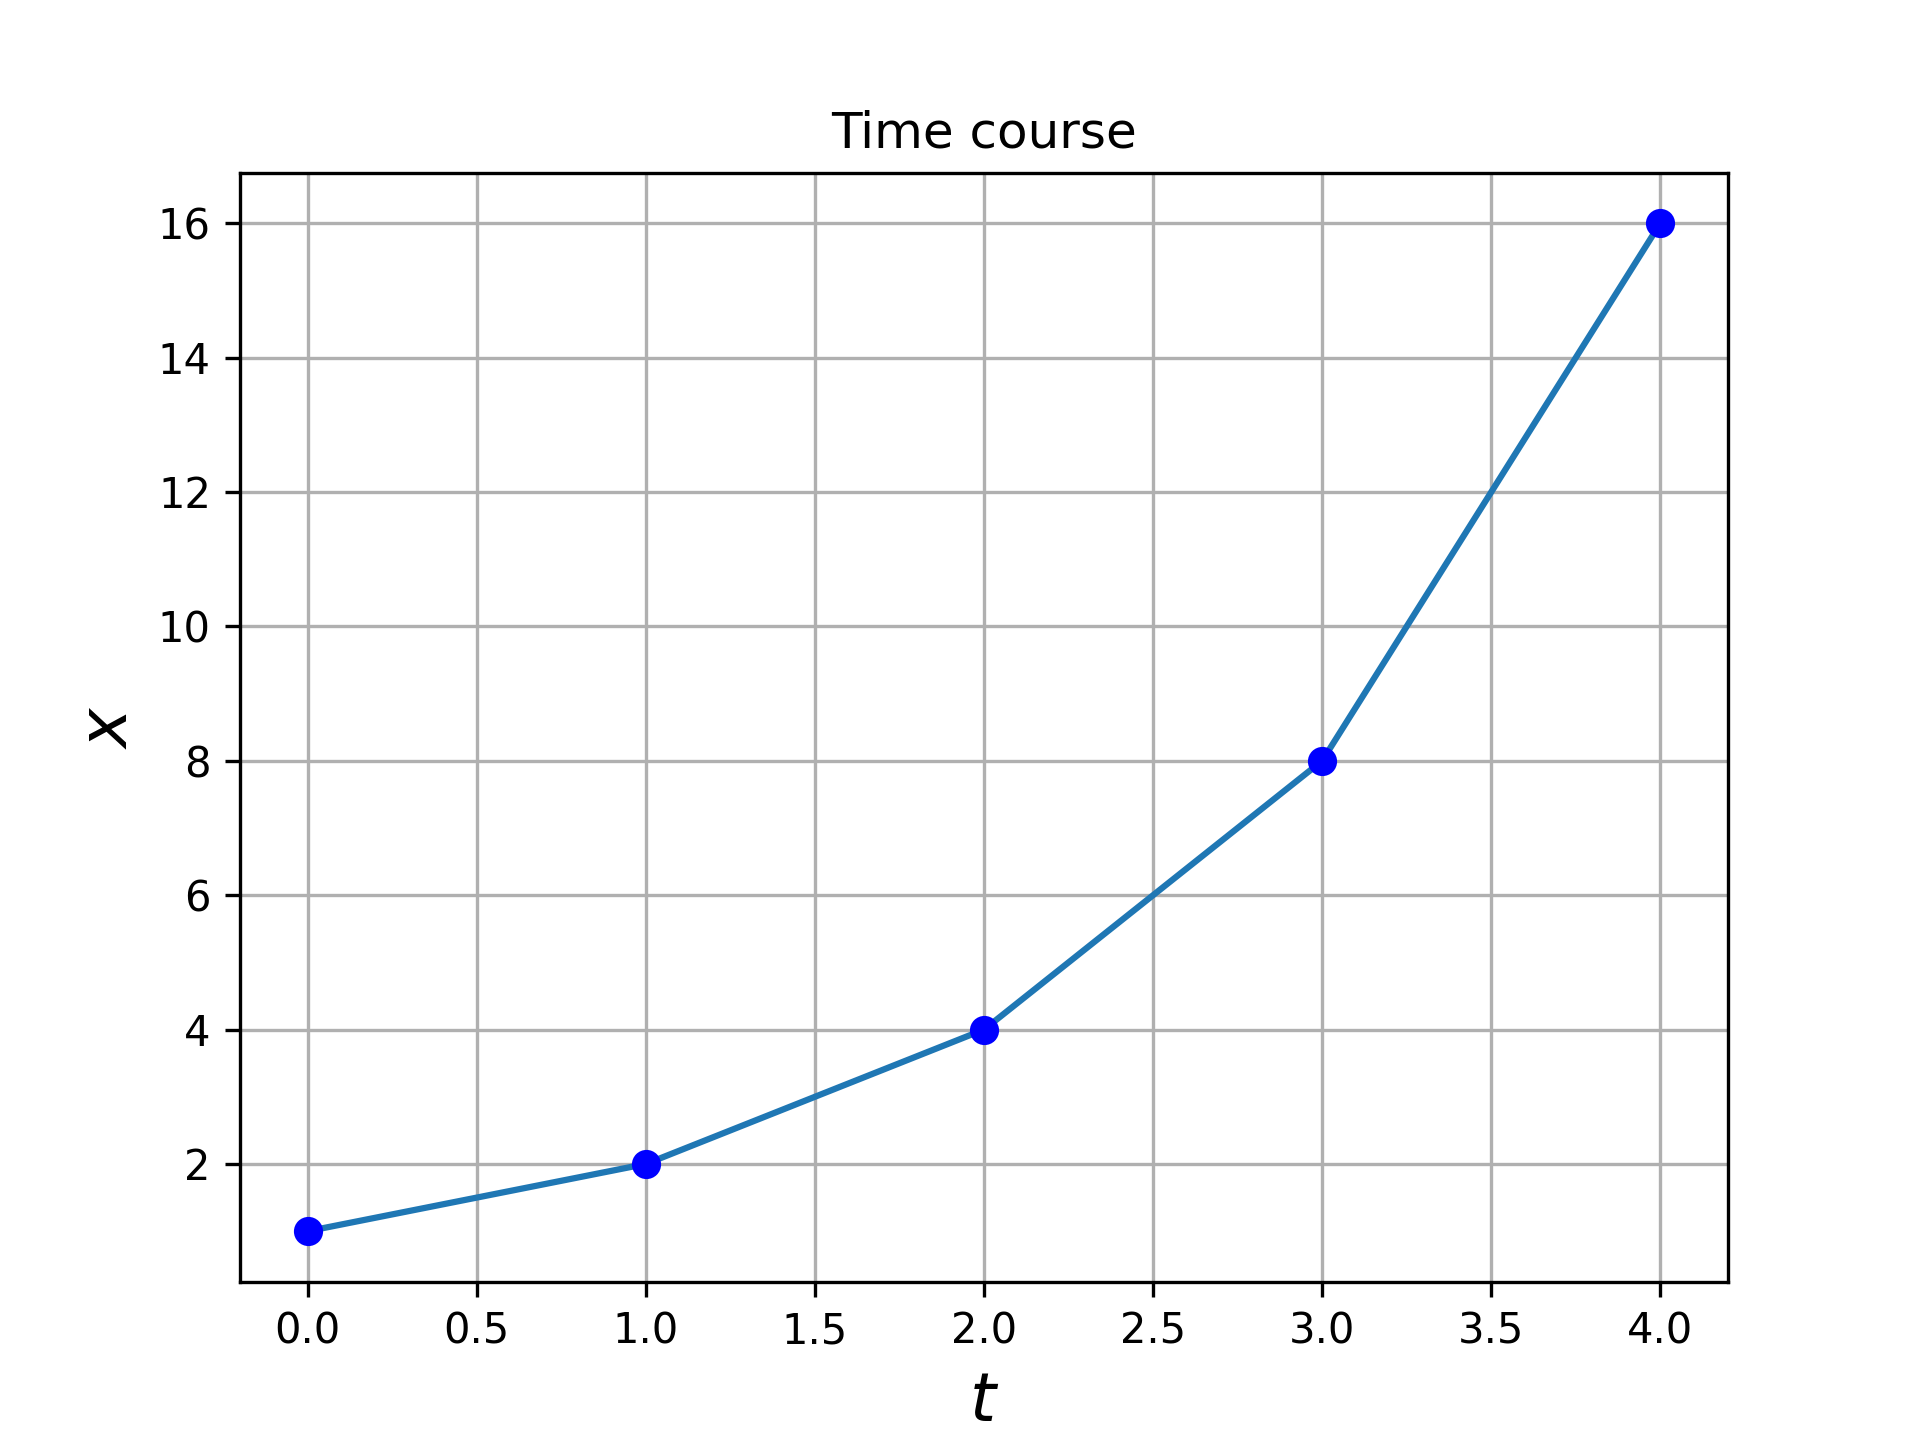
\includegraphics[width=0.46\textwidth]{time_course}
		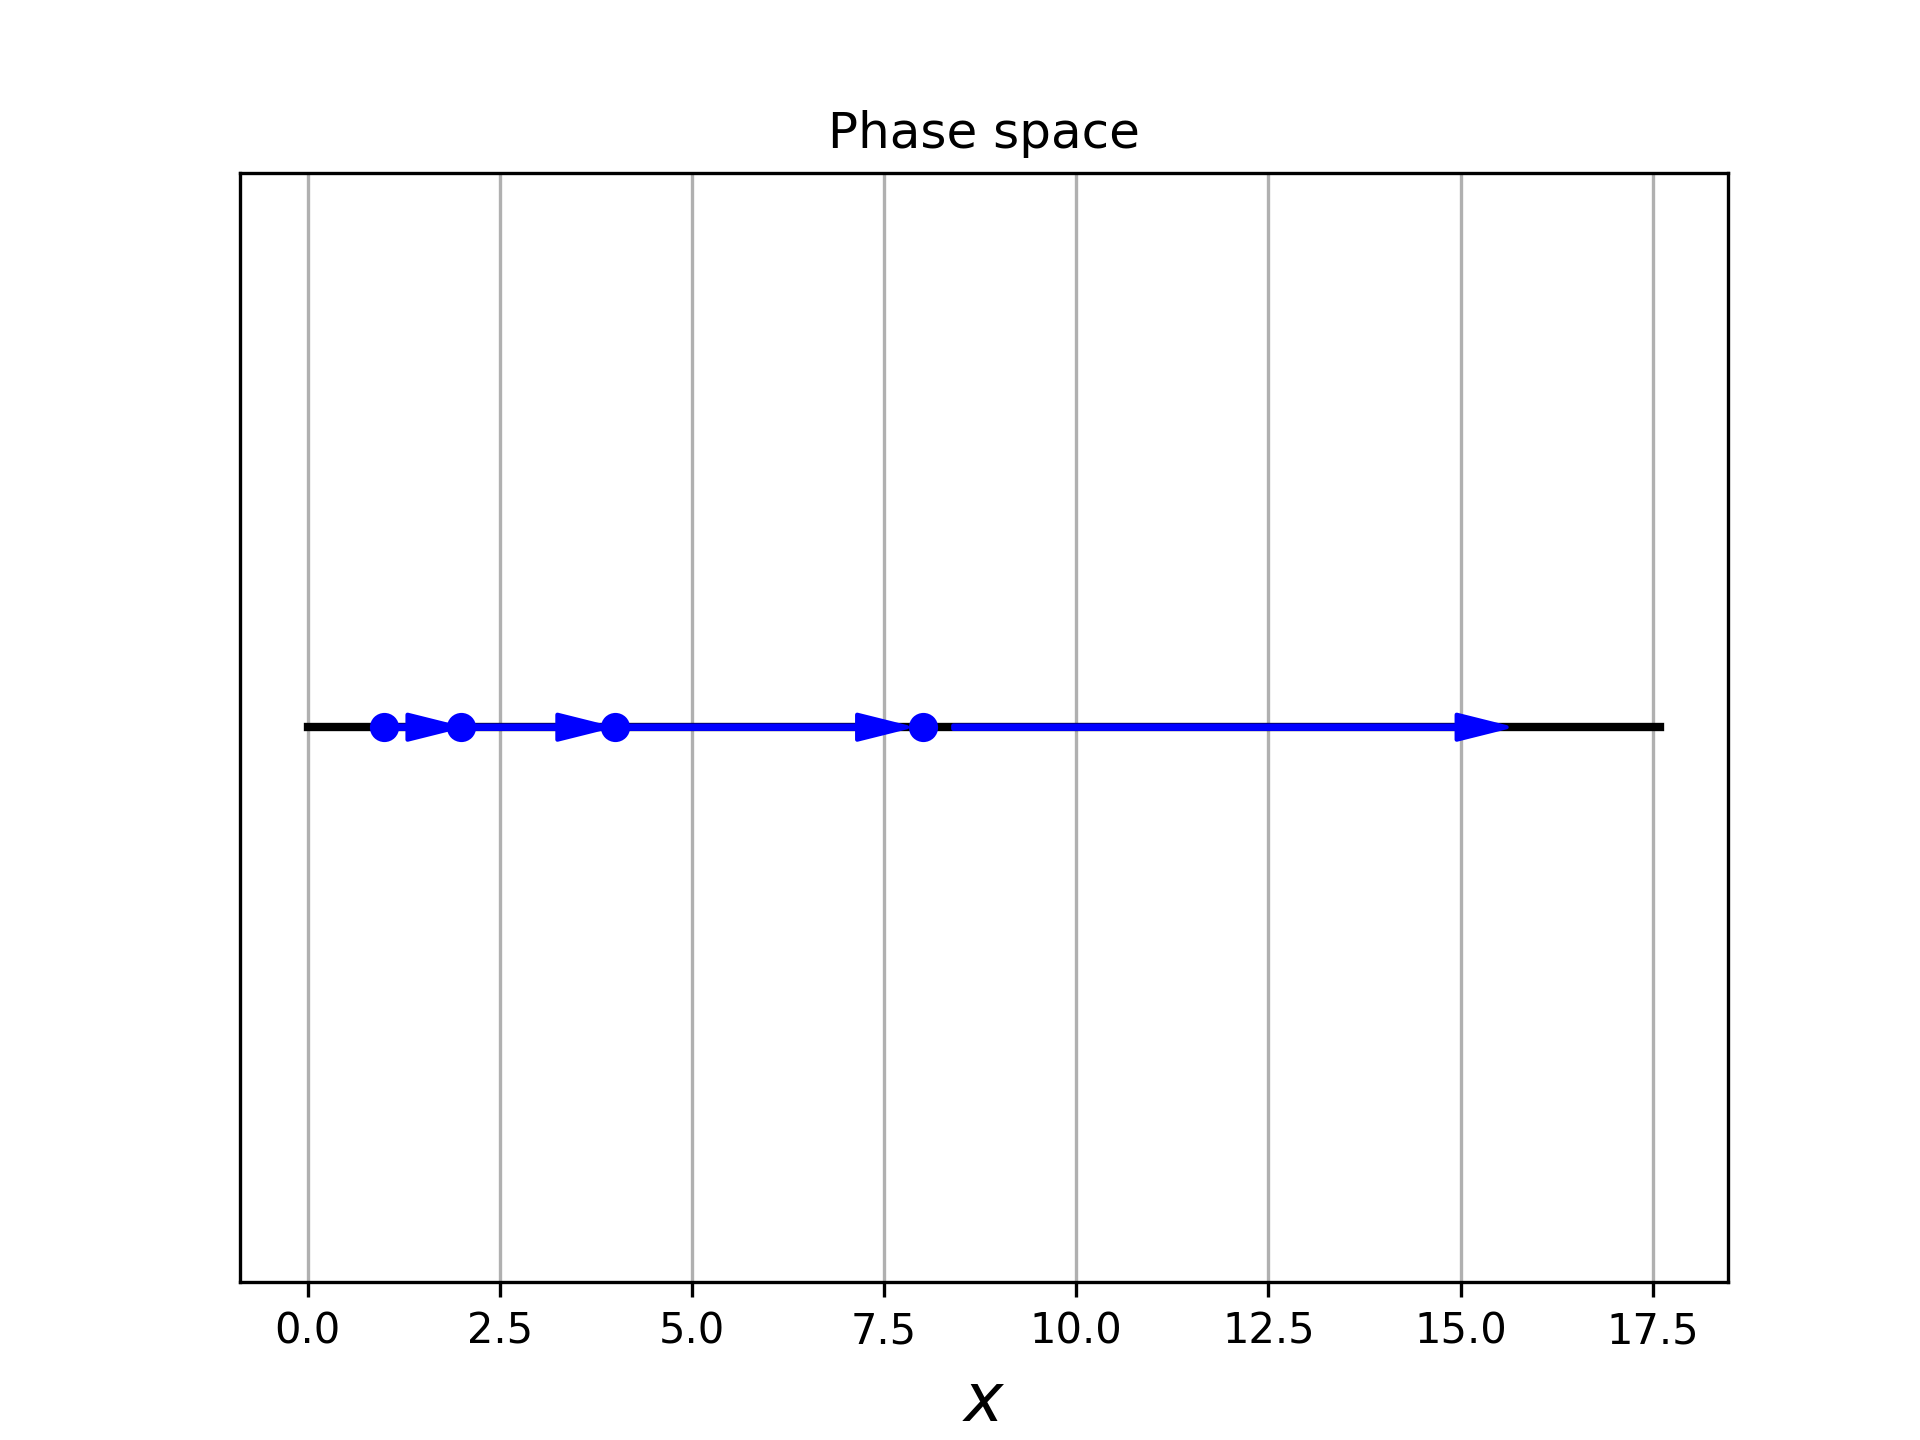
\includegraphics[width=0.46\textwidth]{phase_space}
	\end{center}
	\caption{Dynamics of a population of microbes. The graph on the left shows the time course, $x$ vs $t$ while the graph on the right shows the one-dimensional phase space (a line) where a series of points show the successive values of x as dots. The points are connected by arrows to show the progression. The trajectory followed by a system in phase-space is called an orbit.}
	\label{fig:tcourse}
\end{figure}

 We could just plot the results as the state of our system, $x$, against time, we would call that a time course. For more complex systems, we may prefer to show the state of the system as point in space. For instance, our first mathematical model has a single variable so any  state can be represented as a point on the real line.